\section{Quantum node model}
\label{netqasm:sec:abstract_model}

In this work we will assume an abstract model of the hardware and software architecture of end-nodes in a quantum network.
Specifically, we assume each end-node to consist of a \acf{CNPU} and a \acf{QNPU}.
The \ac{CNPU} can be also be seen as a the user space of a classical computer, and the \ac{QNPU} as a coprocessor.

This model takes into account both physical- and application-level constraints found in quantum network programming.
The \ac{QNPU} can be accessed by the \ac{CNPU}, at the same node, to execute quantum and classical instructions.
We define the capabilities of the \ac{QNPU}, and roughly their internal components, but do not assume how exactly this is implemented.
In the rest of this work, we simply use the \ac{QNPU} as a black box.

The \ac{QNPU} can do both classical and quantum operations, including
    (1) local operations such as classical arithmetic and quantum gates and
    (2) networking operations, i.e. remote entanglement generation.
The \ac{CNPU} cannot do any quantum operations.
It can only do local computation and classical communication with other nodes.
In terms of classical processing power, the difference between the \ac{CNPU} and the \ac{QNPU} is that the \ac{CNPU} can do heavy and elaborate computation, while we assume the \ac{QNPU} to be limited in processing power.

The \ac{CNPU} can interact with the \ac{QNPU} by for example sending instructions to do certain operations.
The \ac{CNPU} and the \ac{QNPU} are logical components and may or may not be the same physical device.
It is assumed that there is low latency in the communication between these components, and in particular that they are physically part of the same node in the network.

One crucial difference between the \ac{CNPU} and the \ac{QNPU} is that the \ac{CNPU} can do application-level classical communication with other end-nodes, while the \ac{QNPU} cannot.
The \ac{QNPU} can communicate classically to synchronize remote entanglement generation, but it does not allow arbitrary user-code classical communication.
We use this restriction in order for the \ac{QNPU} to have relatively few resource requirements.

The \ac{QNPU} consists of the following components, see \cref{fig:qnpu}:
\begin{itemize}
    \item \textbf{Processor:}
            The processor controls the other components of the \ac{QNPU} and understands how to execute the operations specified by the \ac{CNPU}.
            It can read and write data to the classical memory and use this data to make decisions on what operations to do next.
            It can apply quantum gates to the qubits in the quantum memory and measure them as well.
            Measurement outcomes can be stored in the classical memory.
    \item \textbf{Classical memory:}
            Random-access memory storing data produced during the execution of operations, such as counters, qubit measurement outcomes, information about generated entangled pairs, etc.
    \item \textbf{Quantum memory:}
            Consists of communication and storage qubits, see \cref{netqasm:sec:quantum_networks}, on which quantum gates can be applied.
            The qubits can be measured and the resulting outcome stored in the classical memory by the processor.
            The communication qubits are connected through a quantum channel to adjacent nodes in the quantum network, through which they can be entangled.
            This quantum channel may also include classical communication needed for synchronization, phase stabilization or other mechanisms needed in the specific realization.
    \item \textbf{Quantum network stack:}
            Communicates classically with other nodes and quantum repeaters in the network to synchronize the generation of remote entanglement, and issues low-level instructions to execute the entanglement generation procedures, see~\cite{dahlberg2019linklayer,kozlowski2020networklayer}.
\end{itemize}

We stress that the internals of the \ac{QNPU} are not relevant to the design of \ac{NetQASM}.
We do assume that the \ac{QNPU} only has limited classical processing power, and can therefore be implemented on for example a simple hardware board.


% \begin{figure}[t]
%     \centering
%     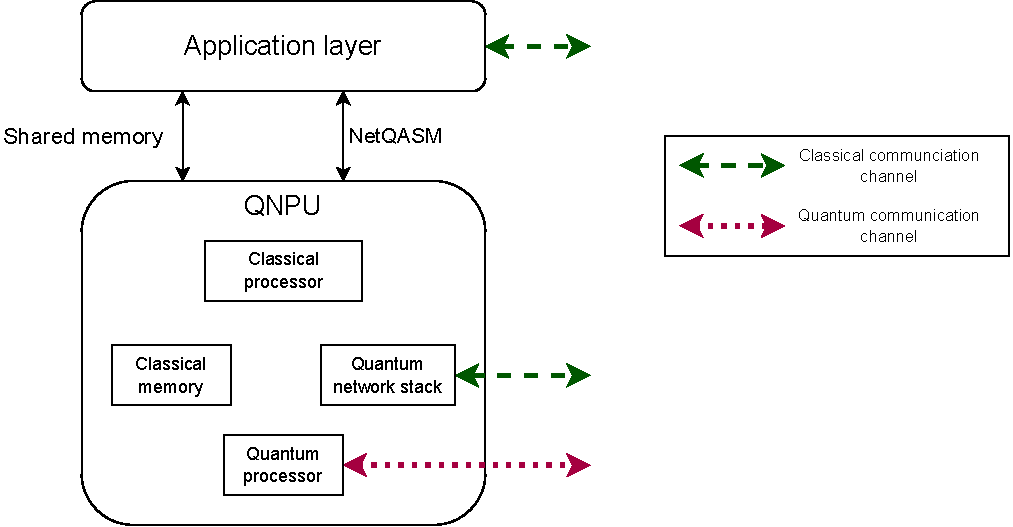
\includegraphics[width=0.6\linewidth]{figures/netqasm/qnpu.pdf}
%     \caption{Overview of \ac{QNPU} components and interfaces. The \ac{CNPU} talks to
%         the \ac{QNPU} using \ac{NetQASM}. The processor inside the \ac{QNPU} can interact with
%         all other components. Channels are connecting components with corresponding
%         components in adjacent nodes in the network.}
%     \label{fig:qnpu}
% \end{figure}



\subsection{Applications and programs}
As mentioned in~\cref{netqasm:sec:introduction}, quantum network \textit{applications} (or protocols) are multi-partite and distributed over multiple end-nodes.
The unit of code that is executed on each of the end-nodes that are part of the application, is called a \textit{program}.
We will use this terminology throughout the rest of the paper.

As mentioned in the previous section, the end-nodes are modeled such that there is an application layer and a \ac{QNPU}. We assume that execution of quantum network programs is handled by the application layer.
How exactly the program is executed, and how the \ac{QNPU} is involved herein, is part of the \ac{NetQASM} proposal.